\begin{figure}[t]
    \centering
    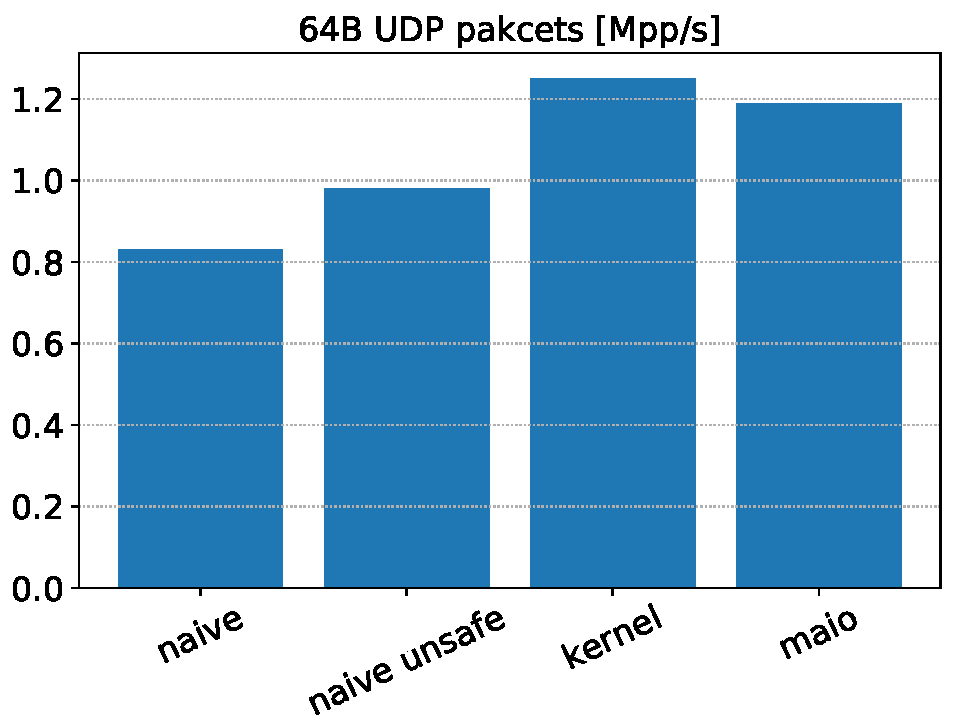
\includegraphics[width=\columnwidth]{syscall.pdf}
    \caption{Number of 64B udp packets sent using user-space sockets(both with and without mitigations), kernel sockets and MAIO.} 
    \label{fig:pps}
\end{figure}
\begin{figure}[t]
    \centering
    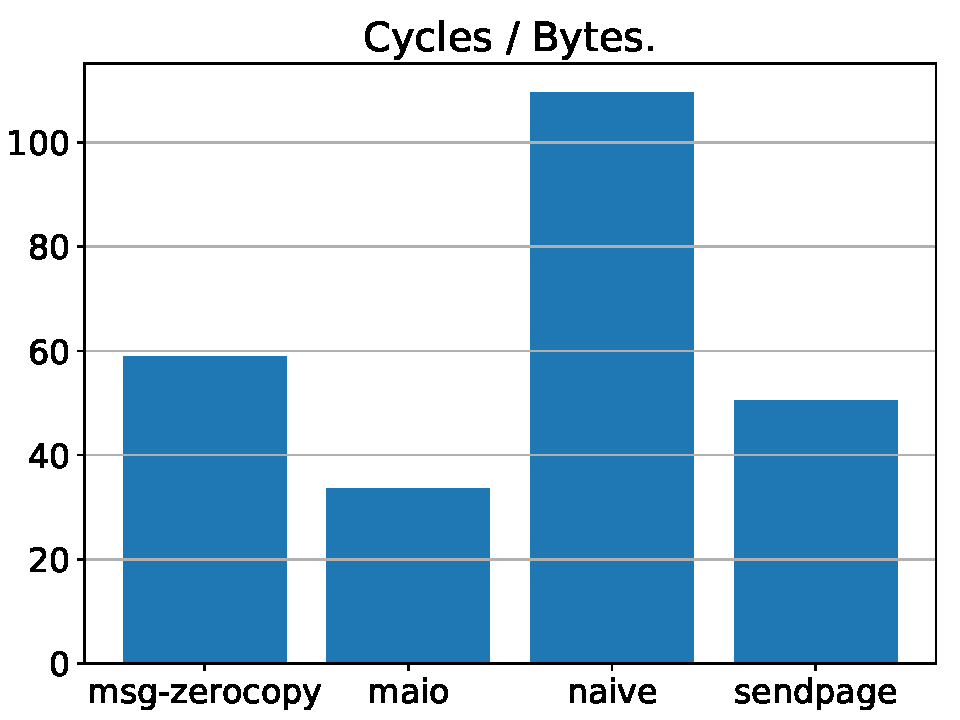
\includegraphics[width=\columnwidth]{send.pdf}
    \caption{The average cycles per packet needed for each zero-copy method (16KB sends). [lower is better]}
    \label{fig:tx_compare}
\end{figure}
\section{Evaluation}
We evaluate the benefits of \oursys on a virtual environment in the Google Clod Platform(GCP).
For our testing we have crated three VMs; 16 core\footnote{These VMs have two threads per physical core} Intel Cascade Lake high-throughput VMs capable of 32Gb/s of egress bandwidth\cite{gcp}, each with 64GB of RAM.

In all experiments we have repeated the test 10 times, and we show the average result. We use perf\cite{perf} to analyze the major contributors to the cycles per byte costs of each of tested techniques.

\subsection{Bifurcated TX}\label{sec:eval_bif}
In this experiment we evaluate the direct benefit of bifurcated system calls. Each program sends a UDP stream of 64 Byte packets. The goal of this experiment is to gauge the impact of system calls on perfromance. We compare a simple \texttt{send\_msg}, a kernel thread performing \texttt{kernel\_send\_msg} and \oursys. We run the naive version twice, once with \texttt{mitigations=off}\cite{mitigations} and once without this boot parameter. We present the number of sent datagrams per second in million packets per second(Mpp/s), the results are shown in Fig \ref{fig:pps}. We see that \texttt{mitigations}(naive unsafe in the figure) have a negative impact of 20\% on the performance of the naive \texttt{send\_msg}. Without mitigations a kernel thread and \oursys still perform better than the naive thread by 25\% and 20\% respectively.

\subsection{Zero Copy TX}
We evaluate the cost of data copying for single sending process. To minimise the impact of system calls on performance we send 16KB buffers. We evaluate a simple \texttt{send\_msg}(i.e., naive), a \texttt{send\_msg} with the \texttt{MSG\_ZERO\_COPY} flag, \texttt{sendfile} and \oursys. In this experiment all the senders were working at the rate of 27Gb/s, but the \texttt{send\_msg}, which was bottle necked on the core CPU and as a result working at the rate of 19Gb/s. The results of the experiment are shown in Fig. \ref{fig:tx_compare}, we show the Cycles/Byte metric as a meter of efficiency. We calculate the metric by measuring the CPU utilisation in CPU cycles and dividing by the total bytes sent per second. In this experiment about 50\% of the CPU cycles for \texttt{send\_msg} were spent on copying data. This amounts to about 55 CPU cycles spent on each sent Byte, we assume this includes memory access. With the \texttt{MSG\_ZERO\_COPY} flag, about 37\% of the CPU cycles are spent on \texttt{get\_user\_pages\_fast}, which translates to 22 cycles spent on dynamic remapping per byte. These results confirm the findings first reported in the original \texttt{MSG\_ZERO\_COPY} paper\cite{desendmsg}. Sendpage, was closer in performance numbers to \texttt{MSG\_ZERO\_COPY} rather than to \oursys, due to the cost of \texttt{splice} abstractions, with 19\% of the cycles spent on \texttt{generic\_file\_splice\_read} and another 7\% spent on call stack from \texttt{generic\_splice\_sendpage} to the actual \texttt{tcp\_sendpage} that performs the TCP send. In the Linux kernel \texttt{send\_msg} is implemented with \texttt{splice} abstractions.

\begin{figure}[t]
    \centering
    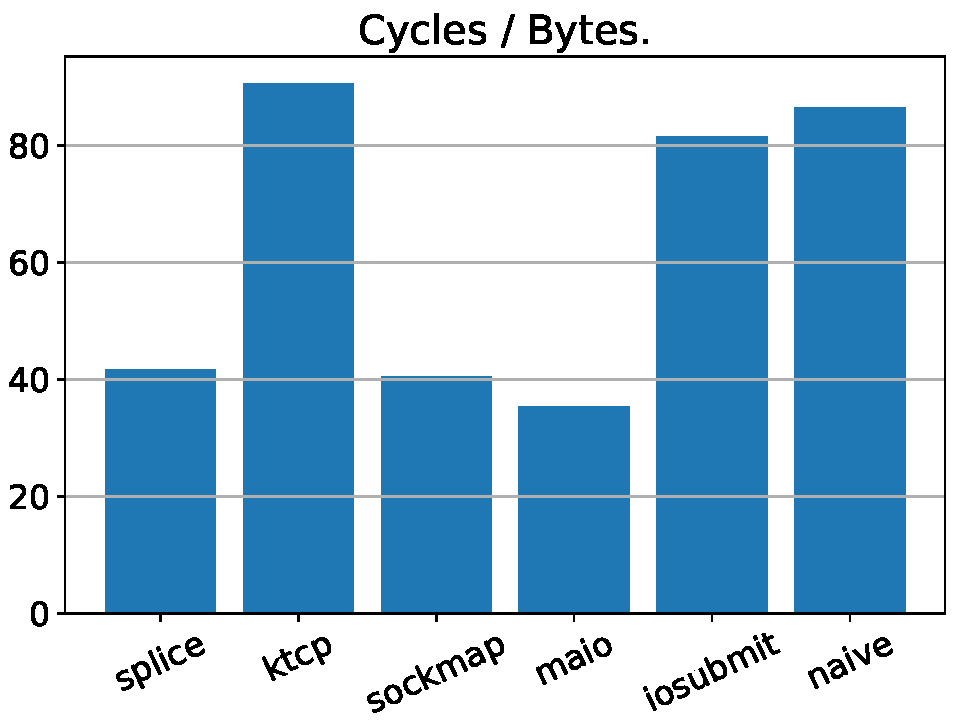
\includegraphics[width=\columnwidth]{splice.pdf}
    \caption{The average cycles per packet needed for each splicing solution. [lower is better]}
    \label{fig:cyc_byte}
\end{figure}

\subsection{Socket Splicing}
We perform a simple TCP socket splicing experiment (i.e., Mvoing bytes from one TCP socket to another) akin to the TCP-split functionality of KTCP. We measure the effectiveness of each proposed solution by looking the the number of CPU cycles spent on average to splice (i.e., receive and send) a single byte. Results are shown in Fig. \ref{fig:cyc_byte}

We use 256KB buffers both for RX and TX, rendering the effect of system calls negligible. System calls account for less than 1\% of the cpu syscalls of iosubmit,splice and naive. Unsurprisingly, KTCP, iosubmit and naive all spend between 25\% to 32\% of the cycles on memory copying. While both splice and sockmap perform much better than the copying functions \oursys is still able outperform both by about 10\%. \oursys has none of the \texttt{splice} abstraction overheads between the actual TCP receive and send and none of the costs associated with eBPF. 

%Why we are \emph{not} touching DPDK and friends with a stick.

%Splice Compare (Check Poll):
%\begin{itemize}
%    \item Naive
%    \item SOCKMAP
%    \item splice
%    \item vmsplice  (?)
%    \item io\_remap (?)
%    \item ktcp - kernel TCP client + halfduplex.
%    \item \oursys - kernel zero TCP client + read/write op. 
%    \item ktcp\_zero. - kernel zero TCP client
%\end{itemize}


%\subsection{BW - cycles/byte}
%\subsection{Latency TCP/RR}
%\subsection{Scale - multiple connections - BW,Latency}